\chapter{Proteins}
\section{What are proteins and why do we care?}
Proteins are the fundamental machines of biology, performing tasks such as catalysis, transporting molecules, or providing the structural backbone of the cell.
They play fundamental roles in the biochemical pathways, so understanding them can lead us to create new and refined drugs,
or bio-engineered bacteria.

%In this chapter I will present the basic vocabulary of protein structures, and give an overview of their biochemistry.

But, how are they created?
The information \marginpar{Protein biosynthesis}
used by the cell to build proteins is encoded in the DNA.
When the biosynthesis begins, the double helix unfolds, and the genetic contact is translated into RNA.
This new molecule is then transported to the ribosomes, the organelles that translate the RNA into functional proteins.


\section{The many levels of protein structures}
Proteins are structured at several levels, depending at the scale we look at them.
In this section, I will present the main descriptions of proteins at different scopes.


\subsection{The amino acids}
Amino acids are the building blocks of proteins.
They are composed of a carboxyl (-$COOH$) and an amine (-$NH_2$) groups, forming the backbone, and a side-chain.
Two examples are illustrated in Figure~\ref{fig:amino_acids}.
\marginpar{Only a few of all amino acids appear in the DNA.}
There are at least 500 known naturally occurring amino acids \citep{500_amino_acids}, of which only twenty different species are usually codified in the DNA.
The differences between most of them are only on the side chain\footnote{Proline's sidechain has a ring connecting with the amine in the backbone.}.

The side chains are the group responsible for the specific physico-chemical properties of the compound, such as hydrophobicity, pH, or electrostatic charge.

The backbone can polymerise, bonding with other amino acids and forming a long chain.
Having a common backbone means that in principle, any amino acid can be connected to any other, which gives proteins a very rich and flexible biochemistry:
for a protein of length $L$ there are $20^L$ possible combinations. %$20/19 (20^L - 1)$

\begin{figure}
\centering
\hfil %
\subcaptionbox{Glutamine (Q) \label{subfig:aminoQ}}{\begin{tikzpicture}
    \node[anchor=south west,inner sep=0] (image) at (0,0) {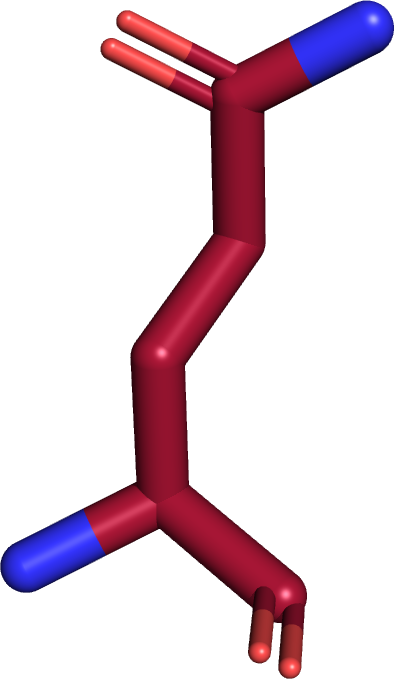
\includegraphics[width=0.25\columnwidth]{bioinfo/figures/amino_acid_Q}};
    \begin{scope}[x={(image.south east)},y={(image.north west)}]
    	\draw[Maroon, thick] (-0.05, -0.05) rectangle (0.85,0.3);
    	\draw[RoyalBlue, thick, dashed] (0.2, 0.35) rectangle (1.05, 1.05);
        %\draw[help lines,xstep=.1,ystep=.1] (0,0) grid (1,1);
        %\foreach \x in {0,1,...,9} { \node [anchor=north] at (\x/10,0) {0.\x}; }
        %\foreach \y in {0,1,...,9} { \node [anchor=east] at (0,\y/10) {0.\y}; }
    \end{scope}
\end{tikzpicture}
} %
\hfil %
\subcaptionbox{Tyrosine (Y) \label{subfig:aminoY}}{\begin{tikzpicture}
    \node[anchor=south west,inner sep=0] (image) at (0,0) {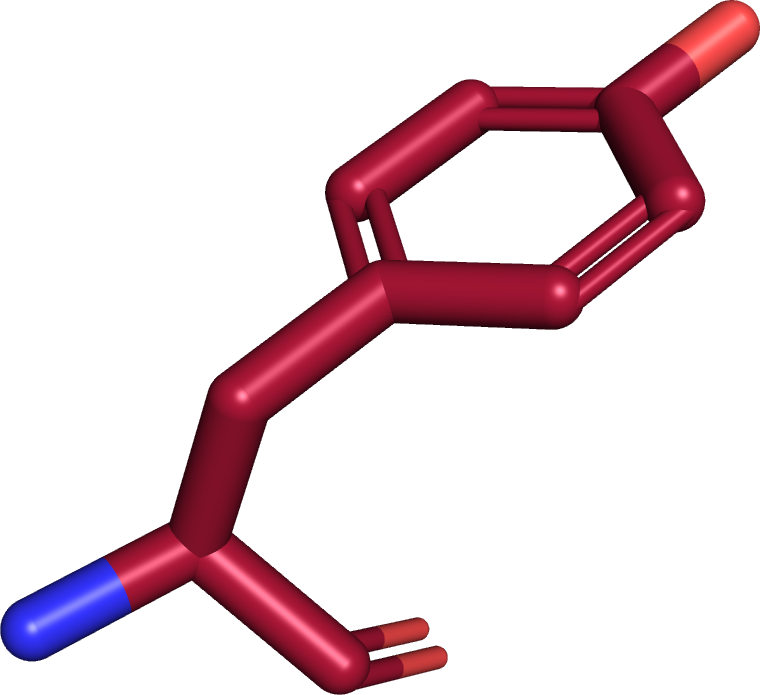
\includegraphics[width=0.45\columnwidth]{bioinfo/figures/amino_acid_Y}};
    \begin{scope}[x={(image.south east)},y={(image.north west)}]
	    \draw[Maroon, thick] (-0.05, -0.05) rectangle (0.6,0.3);
 	    \draw[RoyalBlue, thick, dashed] (0.2, 0.35) rectangle (1.05, 1.05);
        %\draw[help lines,xstep=.1,ystep=.1] (0,0) grid (1,1);
        %\foreach \x in {0,1,...,9} { \node [anchor=north] at (\x/10,0) {0.\x}; }
        %\foreach \y in {0,1,...,9} { \node [anchor=east] at (0,\y/10) {0.\y}; }
    \end{scope}
\end{tikzpicture}
} %
\hfil %
\caption{Two amino acids as appear in proteins.
The \textcolor{Maroon}{maroon}, solid rectangle indicates the backbone, common to all amino acids; and the \textcolor{RoyalBlue}{blue} dashed the side chain, that determines the specific chemical properties.}\label{fig:amino_acids}
\end{figure}

\subsection{Primary structure}
The amino acids can connect to each other through the peptide bond forming a chain.
The \emph{primary structure} is the sequence of amino acids as encoded in the DNA:
\begin{center}
\texttt{ALA ARG ILE ASN GLY ARG GLU ILE ASN VAL THR LYS LYS}
\end{center}

This is the easiest to obtain experimentally, since the advent of next generation sequencing techniques.
The collection of all protein sequences of an organism is the \emph{proteome}.


\subsection{Secondary structure}
The polypeptide chains are locally organised in motifs stabilised by hydrogen bonds.
The most common is the $\alpha$-helix, \marginpar{$\alpha$} shown in Figure~\ref{subfig:alpha}, where the hydrogen bonds are formed between the backbone oxygen of one residue, and the hydrogen of the amine group, four residues beyond, and continued in a regular pattern, forcing the backbone to twist into a helix.
The same bond is possible with residues that are closer -- two or three residues -- or further  -- five residues, the $\pi$ helix -- but are less common.

The second most common arrangement is the $\beta$-sheet  \marginpar{$\beta$} depicted in Figure~\ref{subfig:beta}, where approximately extended chains are placed next to each other and bonds are formed between juxtaposed residues.

\begin{figure}[hb]
	\centering
	\subcaptionbox{$\alpha$-helix\label{subfig:alpha}}{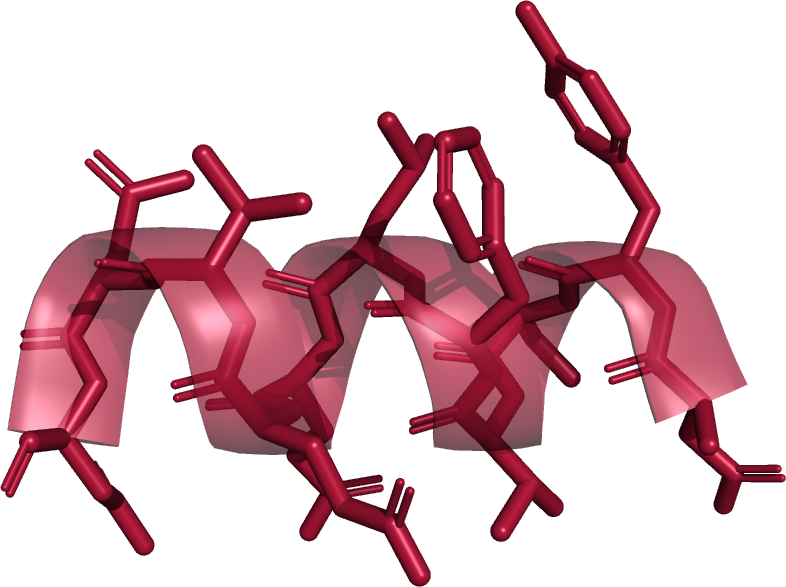
\includegraphics[width=0.9\textwidth]{bioinfo/figures/helix}}\\
	\subcaptionbox{$\beta$-sheet\label{subfig:beta}}{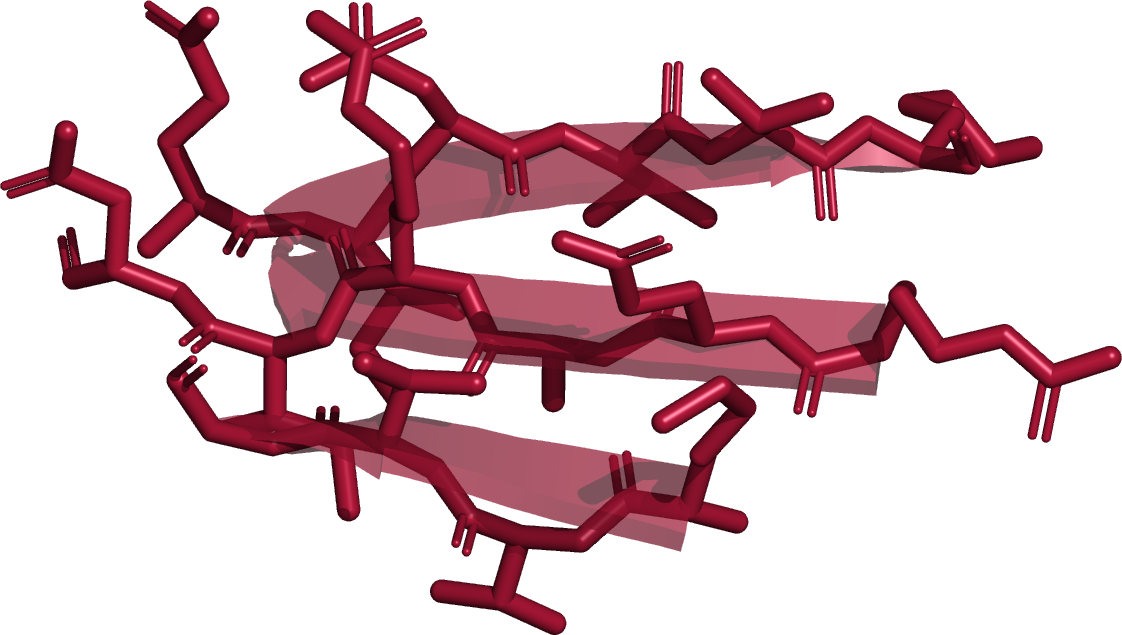
\includegraphics[width=0.9\textwidth]{bioinfo/figures/beta}}
	\caption{The two most frequent secondary structure elements.}\label{fig:alpha_beta}
\end{figure}


\subsection{Tertiary structure}
Once the chain is locally stabilised by the hydrogen bonds it needs to fold into a compact structure.
The spatial arrangement of the secondary structure elements is the \emph{tertiary structure.}
One example is the chain A of the protein \texttt{4V0B}, in Figure~\ref{fig:tertiary}.

\begin{figure}[htb]
\centering
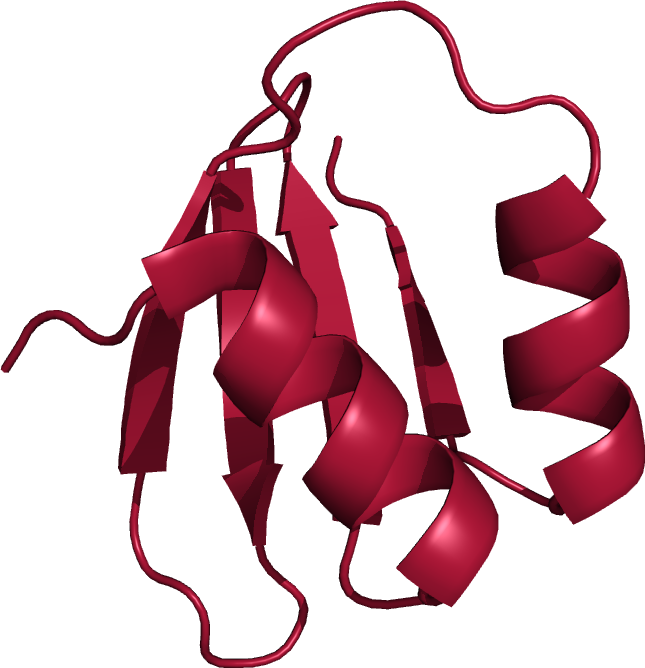
\includegraphics[width=0.8\textwidth]{bioinfo/figures/tertiary}
\caption{Tertiary structure of the chain B of the protein \texttt{4V0B}.}\label{fig:tertiary}
\end{figure}

\subsection{Quaternary structure}
Proteins do not always work alone, but they form complexes composed of several chains.
The relative arrangement of each chain is the quaternary structure.

\begin{figure}[htb]
\centering
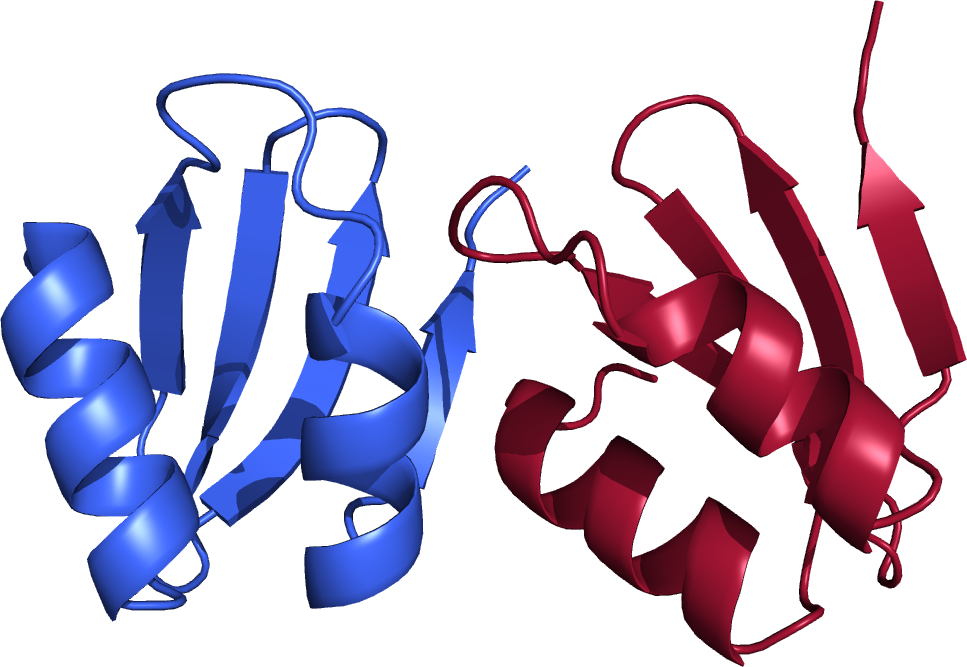
\includegraphics[width=0.8\textwidth]{bioinfo/figures/quaternary}
\caption{Quaternary structure of the chains A and B of the protein \texttt{4V0B}.}\label{fig:quaternary}
\end{figure}

%\subsection{Quintenary structure} %?
\section{Protein biochemistry}

Experiments show that proteins placed in the right medium of pH and temperature will unfold into a random coil, with no trace of tertiary nor secondary structure.
When restored to physiological conditions, they will refold into its natural shape, recovering its original biological and chemical properties.
As long as the protein is chemically unaltered, it will recover the tertiary structure independently of the folding machinery of the cell.
\marginpar{Dogmas that govern protein folding}
This was codified as Anfinsen's dogma: under physiological conditions, the primary structure of globular proteins determines the secondary and tertiary structure, and thus, its function, independently of the cell's machinery \citep{Anfinsen_dogma}.
Typically, the fully folded state is reached in the order of mili- to seconds.
The hypothesis has a few exceptions, namely large, fibrous proteins, prions -- proteins with alternative, stable conformations -- and aggregating proteins -- where the individual proteins bind to each other forming large and non-functional structures.
A reasonable hypothesis is that, a priori, the native conformation seems to be the state in the lowest energy, and the random coil is just rolling down the energy landscape.

\citet{fold_graciously} \marginpar{Levinthal's paradox} noted that, for every amino acid, a protein has two main degrees of freedom corresponding to the torsion of the backbone, plus one more for the rotation of the side chain.
This gives us a configuration space of the order of $10^{2L}$ for a protein of $L$ residues, but the kinematics suggest that it only has time to sample $10^8$ conformations, an exponentially tiny fraction for proteins of typical length.

Levinthal suggested two corrections:
\begin{itemize}
	\item The native conformation is not necessarily the one of minimum energy, but a local minimum with a deep enough well that it is stable.
	\item The native conformation must be kinematically accessible, possibly guided by local interactions that partially fold the protein.
\end{itemize}

These corrections are supported by experiments showing that a certain enzyme only folds at temperatures around 37 C, but it completely stable up to 90 C.
Furthermore, the same enzyme produced by an organism that lives at colder temperatures is shown to require lower temperatures for renaturation, but it is still stable up to 90 C.
The order of events greatly influences the kinetics of folding.

\FloatBarrier
%\subsection{The protein backbone}
\subsection{The hydrophobic effect}

\subsection{Energy terms}
A relatively generic form of the energy dictating the dynamics of a protein is:
\begin{align*}
H(\left\{\vec r_i\right\}_{i=0}^N) =& \underbrace{\sum_{bonds} k_b \left(d - d_0\right)^2}_\alpha + 
\underbrace{\sum_{angles} k_a \left(\theta - \theta_0\right)}_\beta +  \nonumber \\
&+ \underbrace{\sum_{torsions} f\left(\omega\right)}_\gamma +
\underbrace{\sum_{free\ pairs} k_{ij} \left[\left(\frac{r_{0ij}}{r_{ij}}\right)^{12} - 2 \left(\frac{r_{0ij}}{r_{ij}}\right)^{6} \right]}_\delta + \nonumber \\
&+ \underbrace{\sum_{i,j} \frac{q_i q_j}{4 \pi \epsilon r_{ij}}}_\epsilon
\end{align*}
The terms correspond to:

\begin{itemize}
\item[$\alpha$] Harmonic potential on the bond lengths $d$ for every pair of covalent bonded atoms, where $d_0$ is the ideal bond length and $k_b$ is the strength of the potential for the atom types.
\item[$\beta$] Harmonic potential on the angles between adjacent bonds $\theta$.
\item[$\gamma$] Arbitrary function $f$ on every torsion angle $\omega$.
\item[$\delta$] Lennard-Jones potential between all pairs of atoms not covalent bonded, where $r_{0ij}$ denotes the equilibrium distance and $k_{ij}$ the depth of the energy well.
\item[$\epsilon$] Electrostatic energy between charges, assuming they are spherically distributed.
\end{itemize}

Note that the collection $\vec r_i$ % $\left\{\vec r_i\right\}_{i=0}^N$
includes the water molecules and other atoms in the environment of the protein itself.

Of these terms, $\alpha$ and $\beta$ are strictly valid only near their respective minima, while $\delta$ is valid for distances around and beyond the minimum.
In practice, this is not a significant problem because the deviations from the ideal values are small. \marginpar{Dynamics}
From here we can see that most of the dynamics in proteins is given by the flexibility of the torsion angles.
Roughly speaking the torsions on the backbone determine the secondary structure, and the torsions of the side chains determine the packing.

\section{Membrane proteins}

\section{Experimental determination}